\documentclass[letterpaper,12pt]{article}

\usepackage{ge05}
\usepackage{comment}
\usepackage{booktabs}
\usepackage[dvipdfm]{hyperref}
\urlstyle{rm}   % change fonts for url's (from Chad Jones)
\hypersetup{
    colorlinks=true,        % kills boxes
    allcolors=blue,
    pdfsubject={NYU Stern course GB 2303, Global Economy},
    pdfauthor={Dave Backus @ NYU},
    pdfstartview={FitH},
    pdfpagemode={UseNone},
%    pdfnewwindow=true,      % links in new window
%    linkcolor=blue,         % color of internal links
%    citecolor=blue,         % color of links to bibliography
%    filecolor=blue,         % color of file links
%    urlcolor=blue           % color of external links
% see:  http://www.tug.org/applications/hyperref/manual.html
}

\newcommand{\GDP}{\mbox{\em GDP\/}}
\newcommand{\NDP}{\mbox{\em NDP\/}}
\newcommand{\GNP}{\mbox{\em GNP\/}}
\newcommand{\NX}{\mbox{\em NX\/}}
\newcommand{\NY}{\mbox{\em NY\/}}
\newcommand{\CA}{\mbox{\em CA\/}}
\newcommand{\NFA}{\mbox{\em NFA\/}}
\newcommand{\Def}{\mbox{\em Def\/}}
\newcommand{\CPI}{\mbox{\em CPI\/}}

\def\ClassName{The Global Economy}
\def\Category{Class Notes}
\def\HeadName{Business Cycles and Their Properties}

\begin{document}
\thispagestyle{empty}%
\Head

\centerline{\large \bf \HeadName}%
\centerline{Revised: \today}

\bigskip
Over the last two centuries, US real GDP has grown at an average
rate between 3 and 3.5\% a year,
but this growth has been anything but smooth:
annual growth rates over the last fifty years have
ranged from $-2$\% or less (in 1975, 1982, and 2008)
to 8\% (in 1966 and 1985).
These short-term ``fluctuations'' or ``business cycles''
(we'll use the terms interchangeably)
are the subject of intense interest by businesses
and play an important role in their decisions to hire, produce, and invest.
And it's not just the US;
although we will use US data, other economies exhibit similar
volatility.
Emerging markets, including the US in the 19th century,
differ primarily in having greater volatility.
The bottom line:  fluctuations in economic growth
are a fact of life.

Our mission is to outline some of the basic features
of these fluctuations, which point to ways of dealing with
the inevitable risk and uncertainty they bring to our lives.


\subsubsection*{Cycles and volatility}

Arthur Burns and Wesley Mitchell, the pioneers of business cycle research,
noted:  
%
\begin{quote}
{Business cycles are a type of
fluctuation found in the aggregate economic activity of
nations.... A cycle consists of expansions occurring at about the
same time in many economic activities, followed by similarly
general recessions, contractions and revivals which merge into the
expansion phases of the next cycle; this sequence of changes is
recurrent but not periodic; in duration business cycles vary from
more than one year to ten or twelve years.}
\end{quote}
(From: {\it Measuring Business Cycles\/}, NBER, 1946.)

\begin{figure}[h]
    \centering
    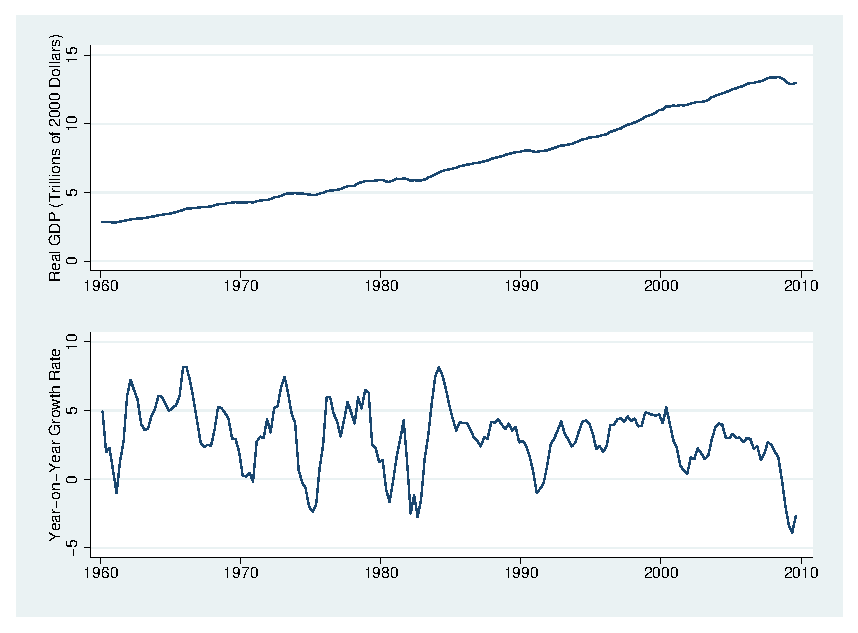
\includegraphics[scale=0.8]{usygy.eps}
    \caption{Level and Fluctuations of US Real GDP.}
    \label{fig:yandgy}
\end{figure}

You can get a sense of these economy-wide fluctuations 
from Figure~\ref{fig:yandgy},
where we plot real GDP and its year-on-year growth rate ---
the rate of growth of quarterly GDP over the same quarter a year earlier.
As someone once said:  the variance is so large that you hardly notice the mean.  
The figure also suggests that volatility was lower between 1985
and 2007.
People used to refer to this as the ``great moderation,''
but that seems less appropriate now.

The National Bureau of Economic Research, 
which dates business cycles in the US, 
defines a recession as ``a significant decline 
in economic activity spread across the economy, 
lasting more than a few months, normally visible in real GDP, 
real income, employment, industrial production, 
and wholesale-retail sales.'' 
Using subjective methods, they identify dates of peaks and troughs.
Less formally, many people use the rule of thumb 
that a recession consists of two consecutive quarters
in which GDP has fallen.
The year-on-year growth rates in the figure don't coincide exactly
with this definition, but you can see the eight official NBER 
recessions since 1960 as sharp downward spikes in GDP growth.

%
%\begin{figure}[h]
%    \centering
%    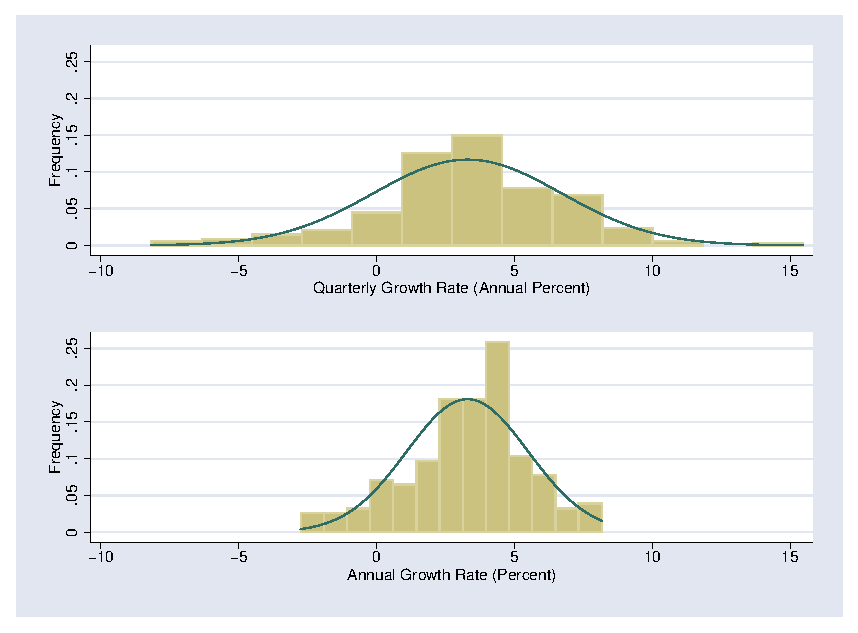
\includegraphics[scale=0.80]{ushist.eps}
%    \caption{Histogram of Fluctuations in US Real GDP.}
%    \label{fig:histogram}%
%\end{figure}
%



\subsubsection*{Expenditure components}

%These recurring fluctuations follow some regular patterns.
Burns and Mitchell refer to fluctuations in
``many economic activities.''
Among these activities are the expenditure
components of GDP.
Are their fluctuations similar to those of GDP?
On the whole, the components, particularly consumption and investment,
move up and down together, but the magnitudes differ enormously.
%Table~\ref{tab:cycleprops} and
%Figure \ref{fig:expenditure_components} document
%these tendencies for the US.

\begin{table}[h!]
\begin{center}
\begin{tabular}{lccc}
\toprule 
        &  Std Dev (\%)  &  Corr w/ GDP  \\
\midrule 
GDP     &      2.19          &    1.00      \\
Consumption:  total      &  1.75  &  0.84   \\
Consumption:  services   &  1.22  &  0.63   \\
Consumption:  nondurable &  1.65  &  0.75   \\
Consumption:  durables   &  6.29  &  0.76   \\
Investment:  total       &  6.64  &  0.86   \\
Investment:  structures  &  7.85  &  0.46   \\
Investment:  equipment   &  7.35  &  0.81   \\
Investment:  housing     &  13.05\phantom{1} &  0.60   \\
Employment               &  1.77  &  0.76   \\
S\&P 500 Index           &  14.98\phantom{1}  &  0.36   \\
\bottomrule 
\end{tabular}
\caption{Properties of Growth Rates.
Numbers refer to year-on-year growth rates
computed from quarterly US data.}
\label{tab:cycleprops}
\end{center}
\end{table}


\begin{figure}[h!]
    \centering
    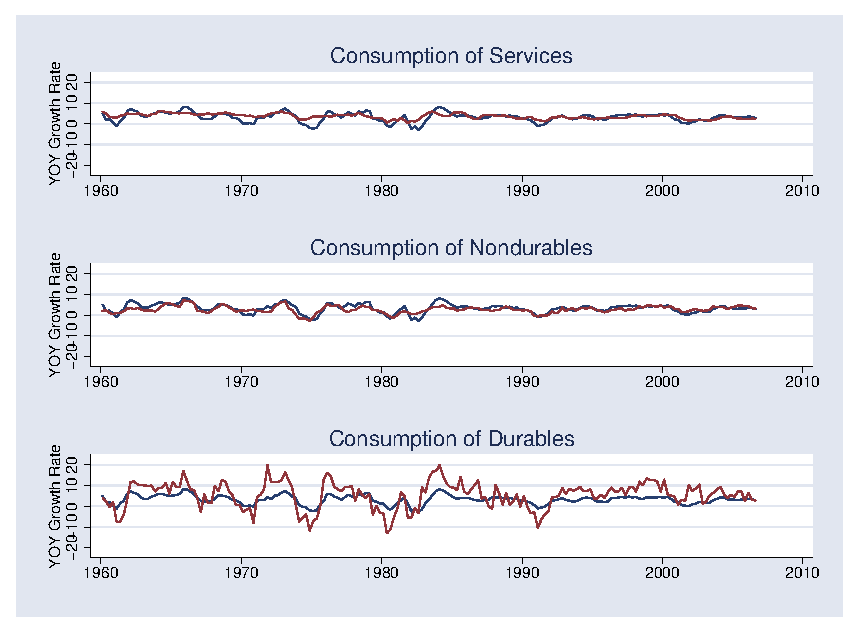
\includegraphics[scale=0.8]{usgcall.eps}
    \caption{Fluctuations in Consumption and GDP.
    The solid (blue) line is real GDP, the other (red) line
    a component of consumption.}
    \label{fig:gcall}%
\end{figure}

\begin{figure}[h!]
    \centering
    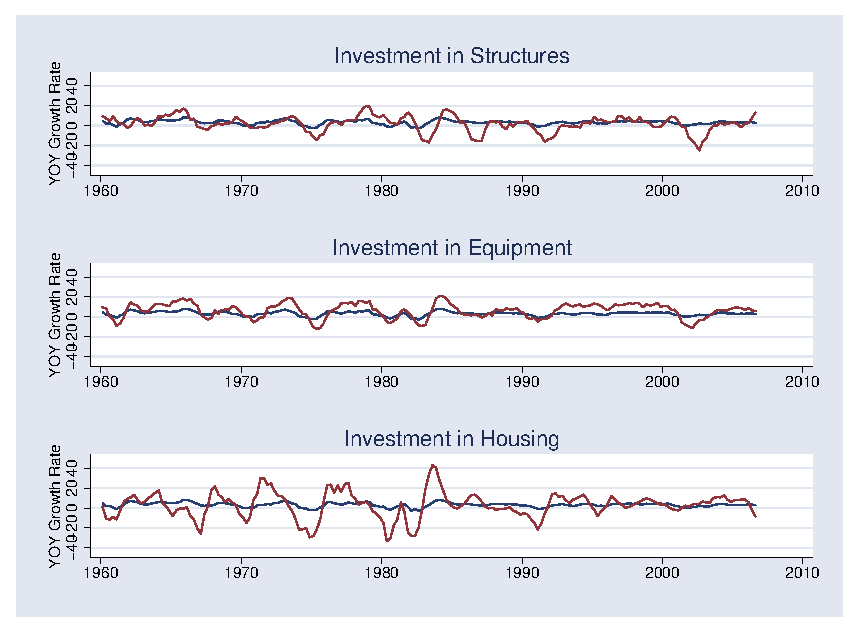
\includegraphics[scale=0.8]{usgiall.eps}
    \caption{Fluctuations in Investment and GDP.
    The solid (blue) line is real GDP, the other (red) line
    a component of investment.}
    \label{fig:giall}%
\end{figure}

Consumption currently accounts for about 70\% of US GDP;
as you might expect, its fluctuations are similar.
The correlation of year-on-year growth rates in consumption (total)
and GDP is 0.84; see Table~\ref{tab:cycleprops}.
Its major components --- services, nondurable goods,
and durable goods --- also vary with GDP,
but their correlations and (esp) volatilities differ somewhat.
Consumption of nondurables and services
is less volatile than GDP, in the sense that
the standard deviation of its growth rate is smaller.
You can see this clearly in Figure~\ref{fig:gcall}.
The dark line in each panel is GDP,
the other line a component of consumption.
It's apparent that consumption of durables is far more
volatile %(in the sense that its standard deviation is larger) 
than consumption of nondurables and services.
You might think of specific products and industries that reflect
the same phenomenon.
Why do you think cars and refrigerators
are more volatile than haircuts and medical care?


Investment (new plant and equipment) also moves up and down with output,
and is substantially more volatile.
As a rule of thumb, a 1\% increase in GDP is associated with
about a 3\% increase in total investment.
(We're looking at the ratio of standard deviations here,
and the high correlation of the two series.)
Table~\ref{tab:cycleprops} and Figure~\ref{fig:giall}
show that the major components --- structures, equipment,
and residential housing --- are highly correlated with,
and more volatile than, GDP.


When we turn to business cycle indicators, we'll see that
many of them are more detailed measures of
some aspect of consumption or investment.
Consumption is important, because it accounts for most of GDP.
Investment is important, because it is highly responsive
to changes in economic conditions.


\subsubsection*{Labor and capital markets move with the cycle}


Labor markets also move with the business cycle ---
indeed, it's the way in which business cycles make themselves 
known to us most directly.  
Figure~\ref{fig:gother} shows how fluctuations in employment
covary with GDP.  
Note that employment growth is generally less than GDP growth;
the difference reflects an increase in output per worker,
a good thing, to be sure!
You can see in the figure that the ups and downs in employment 
typically lag those in GDP by a little --- a quarter or two.  
The current expansion is an extreme case, with 
employment rebounding well before employment, 
but the general pattern is not unusual.  


Aggregate stock prices are extremely volatile, with a standard deviation
about eight times larger than GDP.
The correlation with GDP (0.36) suggests that
good news about the economy is good news for stock prices.
It's hard to see in the figure, 
but we'll see later that stock prices lead GDP:
the correlation of stock prices with GDP two quarters later is above 0.5.
We'll look at this more closely when we turn to indicators.

Labor market indicators and asset prices are
both sources of useful indicators of economy activity.
We'll see more of each in the following section.

%
\begin{figure}
    \centering
    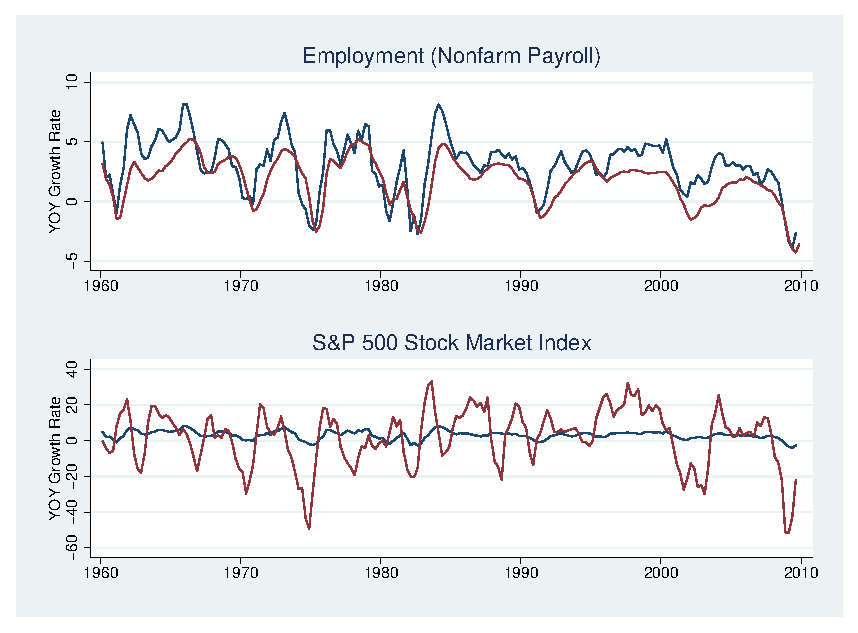
\includegraphics[scale=0.8]{usgother.eps}
    \caption{Fluctuations in Employment and Stock Prices.
    The solid (blue) line is real GDP, the other (red) line
    employment (top panel) or the S\&P 500 Index (bottom).}
    \label{fig:gother}%
\end{figure}


\subsubsection*{Executive summary}

\begin{enumerate}
\item Economies do not grow smoothly:  they exhibit lots of 
short-term volatility.  

\item Spending on investment goods (by firms) 
and consumer durables (by households) are more volatile
 than output.  
 Household spending on nondurable goods and services
 is less volatile than output.  

\item Most variables are procyclical: they move up and down with GDP.  
Examples include consumption, investment, employment, and the stock market.  

\end{enumerate}


\begin{comment}
\subsubsection*{Review questions}

Think about each of the following questions, which we'll address
at greater length shortly:
%
\begin{enumerate}
\item Why do you think consumption is less volatile than output?
Investment more volatile?

%\item Why does employment lag output?

\item Why does the stock market lead output?

\item Why do interest rates typically rise during an expansion?
\end{enumerate}


\subsubsection*{If you're looking for more}

These basic features of business cycles are covered in most
macroeconomics textbooks.  
\end{comment}


\vfill \centerline{\it \copyright \ \number\year \ NYU Stern
School of Business}

\end{document}
